\setlength{\columnsep}{3pt}
\begin{flushleft}
	\begin{itemize}
		\item \textbf{Modem \& Router}: 
		\begin{itemize}
			\item \textbf{Modem}: Send or receive \textbf{data over telephone or cable lines}.
			\item \textbf{Router}: \textbf{Supply the Internet connection} provided by modem to your wired \& wireless devices.
			\begin{figure}[h!]
				\centering
				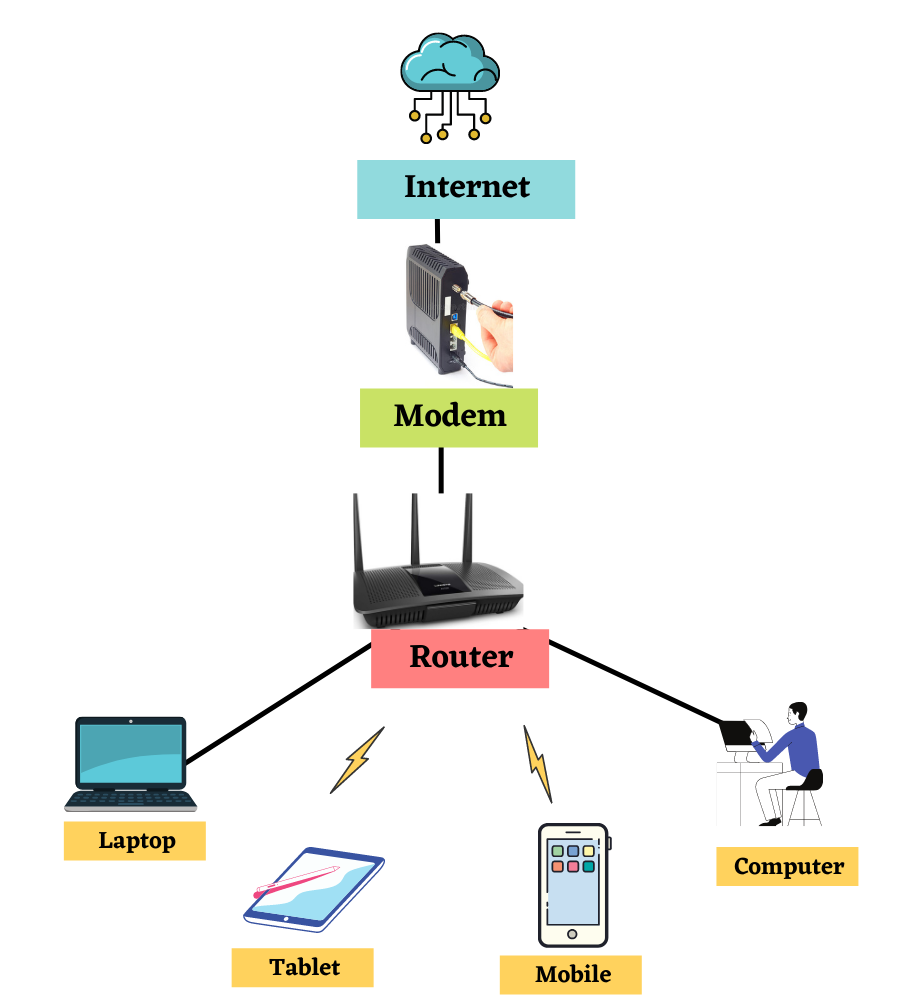
\includegraphics[scale=0.6]{content/chapter14/images/modem_internet.png}
				\caption{Modem \& router}
				\label{fig:modem_router}
			\end{figure}
		\end{itemize}
		\newpage
		\item \textbf{Router \& Switch}: 
		\begin{itemize}
			\item \textbf{Router}: Used for inter-network communication.
			\item \textbf{Switch}: A switch is used to provide additional ports, expanding the capability of the router.
			\begin{figure}[h!]
				\centering
				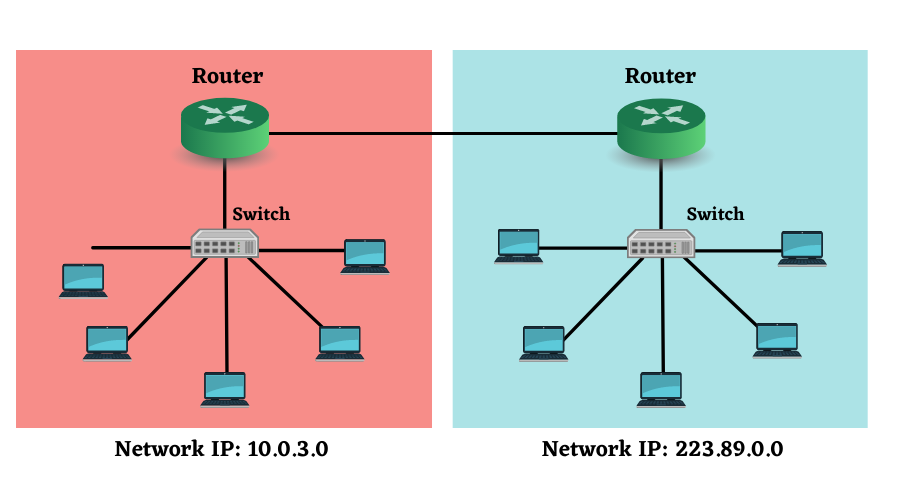
\includegraphics[scale=0.6]{content/chapter14/images/router_switch.png}
				\caption{Router \& Switch}
				\label{fig:router_switch}
			\end{figure}
		\end{itemize}
		\newpage
		\item \textbf{RJ45 Connector}: 
		\begin{itemize}
			\item RJ45 stands for \textbf{Registered Jack 45}.
			\item 8-pin jack used to \textbf{connects a computer to a local area network (LAN)}.
			\begin{figure}[h!]
				\centering
				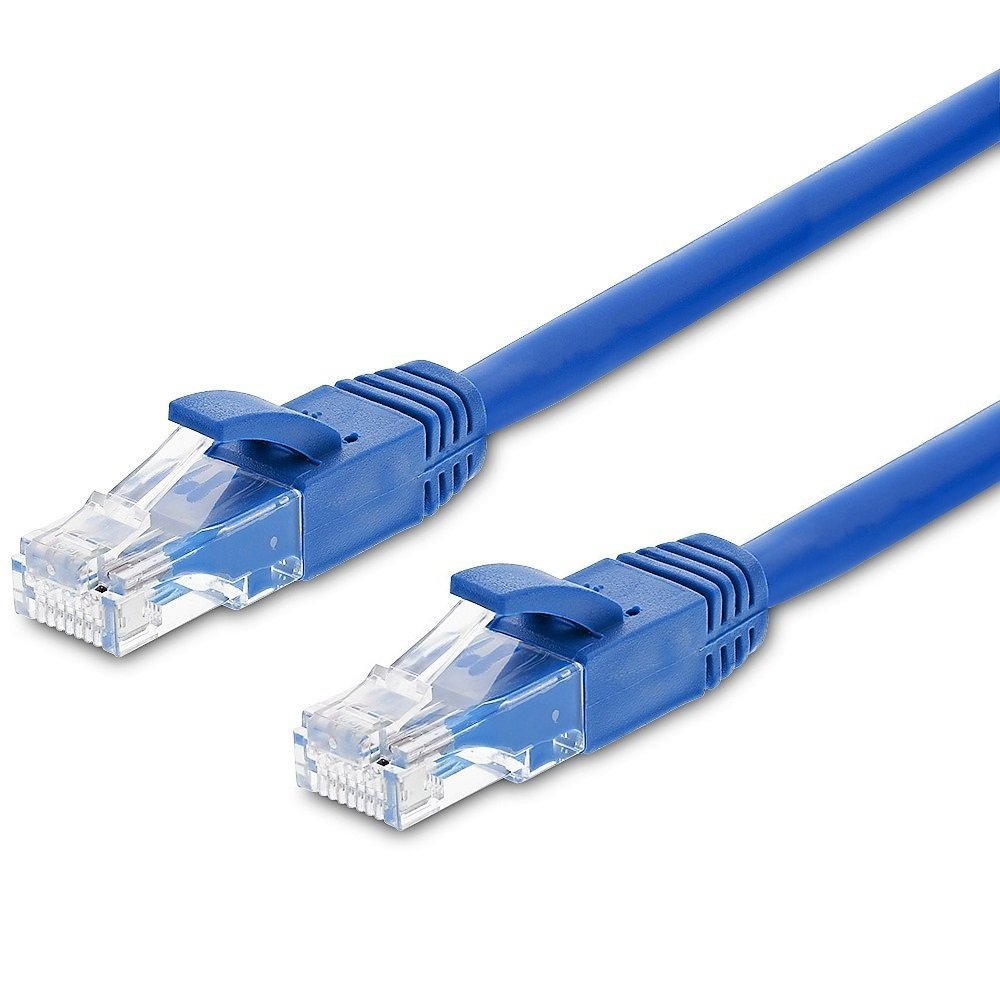
\includegraphics[scale=0.2]{content/chapter14/images/rj45.jpg}
				\caption{RJ45 connector}
				\label{fig:network}
			\end{figure}
		\end{itemize}
		\newpage
		\item \textbf{Ethernet card or NIC}: 
		\begin{itemize}
			\item \textbf{Also called a "network interface card" (NIC)}.
			\item A card that \textbf{plugs into a slot on the motherboard and enables a computer to access an Ethernet network (LAN)}.
			\begin{figure}[h!]
				\centering
				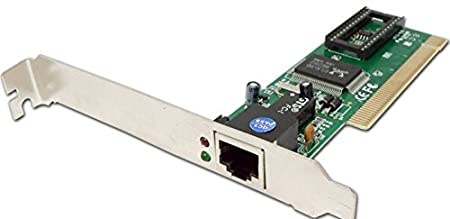
\includegraphics[scale=0.25]{content/chapter14/images/ethernet.jpg}
				\caption{NIC}
				\label{fig:nic}
			\end{figure}
			\item \textbf{Every NIC have a MAC address}: 
			\begin{itemize}
				\item MAC address stands for \textbf{Media Access Control} address
				\item It is a \textbf{unique 48 bit} number identifier assigned to network interfaces card (NIC)
				\begin{figure}[h!]
					\centering
					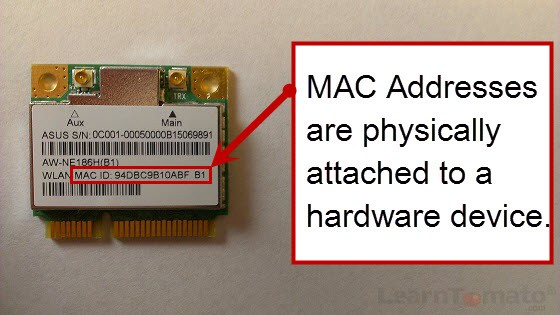
\includegraphics[scale=0.3]{content/chapter14/images/mac.jpg}
					\caption{Mac address}
					\label{fig:mac}
				\end{figure}
				\item Eg of MAC address: \textbf{FF.01.AA.EE.4F.ED}
				\item \textbf{ifconfig} command displays the MAC address of NIC card.
				\begin{figure}[h!]
					\centering
					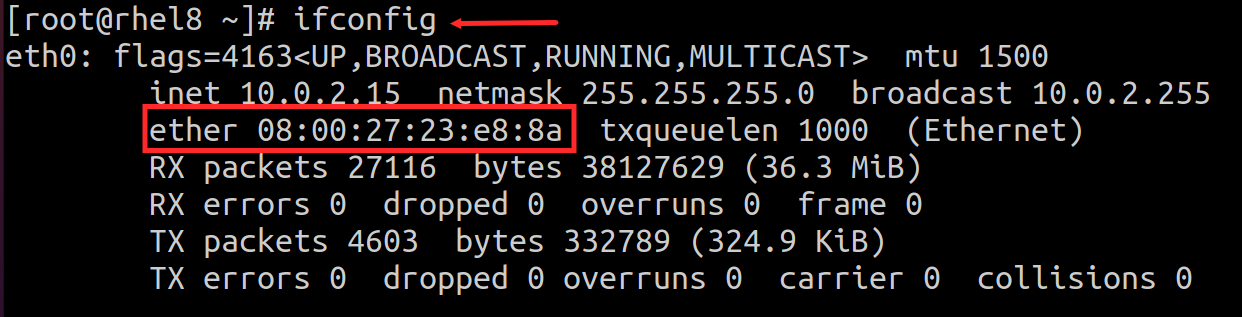
\includegraphics[scale=0.2]{content/chapter14/images/mac.png}
					\caption{MAC address}
					\label{fig:mac_3}
				\end{figure}
			\end{itemize}
		\end{itemize}
		\newpage
		\item \textbf{Gateway}: 
		\begin{itemize}
			\item Used to connect 2 different networks with each other.		
			\item By default, the router acts as default gateway for all the PC in the network. 
				\begin{figure}[h!]
					\centering
					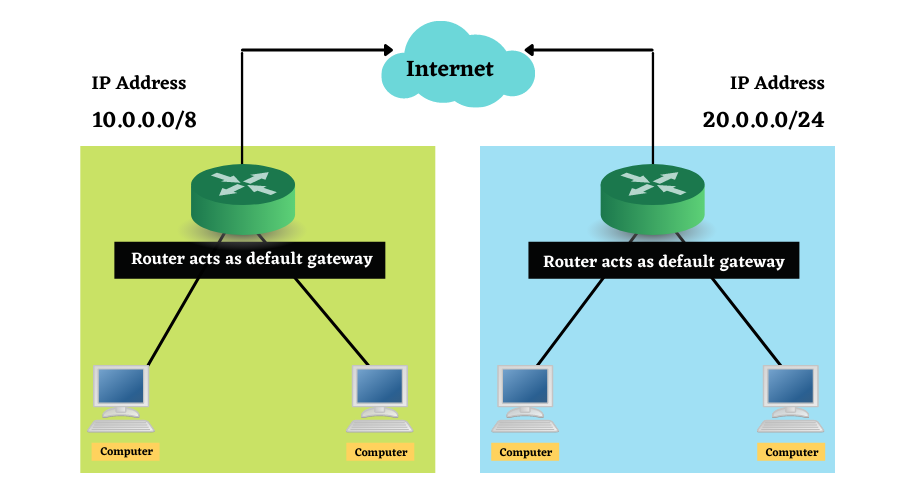
\includegraphics[scale=0.6]{content/chapter14/images/gateway.png}
					\caption{Gateway}
					\label{fig:gateway}
				\end{figure}
		\end{itemize}	
	\end{itemize}
	
\end{flushleft}
\newpage


